\chapter{Methods}\label{sec:MM}
\markright{\thechapter~Materials and methods}

\section{Slab configurator}

The computational work of this thesis is based on the \textit{Slab Configurator}, a Python-based design and optimisation framework initiated by the Sustainability in Structural Design Team of \textit{kfmResearch} \cite{kfmResearch2026}. The original code base provided the general structure for material-based structural assessment and environmental comparison. Within this thesis, the configurator was further developed to extend the considered slab systems, to improve the structural verification models and to enable a consistent comparison of structural and non-structural floor build-ups.

\noindent The overall workflow is shown schematically in Fig.~\ref{fig:slab_configurator_workflow}. The calculation starts with the material and product database. Based on the selected slab system, a cross-section object is created from the available materials and geometric start values. The cross-section is then combined with a member object, which defines the structural system, span, loading and requirements. The member is verified in ultimate limit state (ULS), serviceability limit state (SLS), fire and acoustics. If the selected cross-section does not satisfy the governing requirements, the optimiser modifies the cross-section parameters until a suitable design is found.

\begin{figure}[htbp]
    \centering
    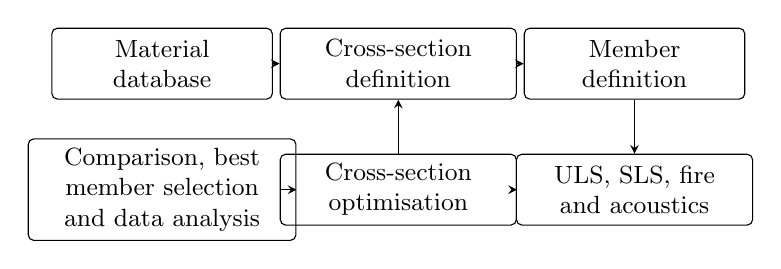
\begin{tikzpicture}[>=stealth, every node/.style={font=\small}]
        \node[draw, rounded corners=2pt, align=center, minimum width=28mm, minimum height=9mm] (db) at (0,0) {Material\\database};
        \node[draw, rounded corners=2pt, align=center, minimum width=30mm, minimum height=9mm] (cs) at (3.0,0) {Cross-section\\definition};
        \node[draw, rounded corners=2pt, align=center, minimum width=28mm, minimum height=9mm] (mem) at (6.0,0) {Member\\definition};
        \node[draw, rounded corners=2pt, align=center, minimum width=30mm, minimum height=9mm] (check) at (6.0,-1.6) {ULS, SLS, fire\\and acoustics};
        \node[draw, rounded corners=2pt, align=center, minimum width=30mm, minimum height=9mm] (opt) at (3.0,-1.6) {Cross-section\\optimisation};
        \node[draw, rounded corners=2pt, align=center, minimum width=34mm, minimum height=9mm] (out) at (0,-1.6) {Comparison, best\\member selection\\and data analysis};

        \draw[->] (db) -- (cs);
        \draw[->] (cs) -- (mem);
        \draw[->] (mem) -- (check);
        \draw[->] (check) -- (opt);
        \draw[->] (opt) -- (out);
        \draw[->] (opt.north) -- (cs.south);
    \end{tikzpicture}
    \caption{General workflow of the slab configurator.}
    \label{fig:slab_configurator_workflow}
\end{figure}

\noindent The comparison is carried out in two stages. First, each slab system is optimised for the selected design criterion and span. Second, the resulting feasible members are post-processed to compare structural quantities and total floor quantities. The structural quantities only include the load-bearing cross-section, while the total quantities additionally include the automatically generated floor build-up required to satisfy the acoustic requirements. The following quantities are evaluated per square metre:

\begin{table}[htbp]
    \centering
    \begingroup
    \small
    \setlength{\tabcolsep}{4pt}
    \renewcommand{\arraystretch}{1.15}
    \begin{tabularx}{\textwidth}{@{}l|l|l|X@{}}
    \hline
    \textbf{Name} & \textbf{Parameter} & \textbf{Unit} & \textbf{Reason} \\ \hline
    Global warming potential &
    $GWP_{\mathrm{struct}}$, $GWP_{\mathrm{tot}}$ &
    kg CO$_2$-eq/m$^2$ &
    Environmental impact of the cross-section and complete floor build-up while accounting for product-specific material variations; see Sec.~\ref{Sec: SustainabilityAss}. \\
    Height &
    $h_{\mathrm{struct}}$, $h_{\mathrm{tot}}$ &
    m &
    Indirect influence on total building height and material demand; see Sec.~\ref{Sec: IndirectInfl}. \\
    Mass &
    $m_{\mathrm{struct}}$, $m_{\mathrm{tot}}$ &
    kN/m$^2$ &
    Indirect influence on foundations, vertical load-bearing structure and seismic mass; see Sec.~\ref{Sec: IndirectInfl}. \\
    Cost &
    $cost_{\mathrm{struct}}$, $cost_{\mathrm{tot}}$ &
    CHF/m$^2$ &
    Economic sustainability and market competitiveness; see Sec.~\ref{Sec: ConstructionCost}. \\
    Construction time &
    $T_{\mathrm{struct}}$, $T_{\mathrm{tot}}$ &
    h/m$^2$ &
    Productivity and construction efficiency; see Sec.~\ref{Sec: Productivity}. \\ \hline
    \end{tabularx}
    \endgroup
    \caption{Sustainability factors for slab comparison.}
    \label{tab:sustainability_factors_slab_comparison}
\end{table}

\noindent The slab configurator is used as a comparative design tool. It does not replace a detailed project-specific structural design, but it enables a consistent assessment of the relative influence of slab system, span, material choice, acoustic build-up and governing design criterion.

\subsection{Material database}

The material database was selected by the Sustainability in Structural Design Team of \textit{kfmResearch} \cite{kfmResearch2026}. It contains mechanical material properties and product-specific environmental data. Environmental Product Declarations (EPDs) are stored on product level and are linked to the mechanical property classes used by the structural models. The database therefore allows a distinction between mechanical performance and producer-specific environmental impact.

\noindent For concrete, reinforcement steel, prestressing steel and timber products, the database stores product density, total GWP, cost and construction time. The implemented calculation converts the product GWP from kg CO$_2$-eq/t to kg CO$_2$-eq/kg and multiplies it by the product density and material volume. The structural GWP per square metre is generally calculated as:

\[
    GWP_{\mathrm{struct}}
    =
    \sum_i
    V_i \rho_i GWP_i
\]

\noindent where $V_i$ is the material volume per square metre, $\rho_i$ is the density and $GWP_i$ is the product-specific global warming potential per kilogram. Cost and construction time are calculated analogously from product-specific cost and construction-time factors.

\noindent The actual GWP range of the products used in the database is summarised in Table~\ref{tab:product_specific_gwp_values}. In the final comparison, material variation is generated by selecting the best and worst available EPD by GWP within each mechanical property group. Thus, for example, concrete strength class C30/37 is sampled with its lowest and highest available product-specific GWP, but it is not mixed with another strength class.

\begin{table}[htbp]
    \centering
    \begingroup
    \scriptsize
    \setlength{\tabcolsep}{3pt}
    \renewcommand{\arraystretch}{1.12}
    \begin{tabularx}{\textwidth}{@{}l|l|c|r|r@{}}
    \hline
    \textbf{Material} & \textbf{Mechanical property} & \textbf{Products} & \textbf{$GWP_{\min}$} & \textbf{$GWP_{\max}$} \\
    & & & kg CO$_2$-eq/t & kg CO$_2$-eq/t \\ \hline
    Ready-mixed concrete & C20/25 & 7 & 77.0 & 102.4 \\
    Ready-mixed concrete & C25/30 & 8 & 75.4 & 100.1 \\
    Ready-mixed concrete & C30/37 & 9 & 76.7 & 104.2 \\
    Reinforcing steel & B500B & 18 & 352.9 & 922.7 \\
    Prestressing steel & Y1860 & 9 & 389.0 & 2250.0 \\
    Glue-laminated timber & GL24h & 21 & -1534.9 & 765.5 \\
    Solid structural timber & C24 & 10 & 75.7 & 363.0 \\
    3- and 5-ply wood & C24 & 13 & -66.2 & 556.0 \\
    3- and 5-ply wood & GL24h & 3 & 250.0 & 415.6 \\ \hline
    \end{tabularx}
    \endgroup
    \caption{Product-specific GWP values stored in \texttt{database\_260126.db}. Negative values occur for timber products where biogenic carbon storage is included in the reported product-specific GWP.}
    \label{tab:product_specific_gwp_values}
\end{table}

\noindent Cost and construction-time assumptions are also stored in the database and are used consistently for all systems. Additional assumptions introduced in the configurator are listed in Table~\ref{tab:cost_time_assumptions}.

\begin{table}[htbp]
    \centering
    \begingroup
    \scriptsize
    \setlength{\tabcolsep}{3pt}
    \renewcommand{\arraystretch}{1.15}
    \begin{tabularx}{\textwidth}{@{}l|X|X@{}}
    \hline
    \textbf{Item} & \textbf{Cost handling} & \textbf{Construction-time handling} \\ \hline
    Concrete, timber, reinforcing steel and prestressing steel &
    Product-specific cost from database multiplied by material quantity per m$^2$. &
    Product-specific construction time from database multiplied by material quantity per m$^2$. \\
    Flat concrete and post-tensioned slabs &
    Additional flat-slab formwork surcharge of 75 CHF/m$^2$. &
    Additional scaffold/formwork time of 0.7 h/m$^2$. \\
    Ribbed concrete &
    Formwork surcharge applied twice to account for the ribbed geometry. &
    Scaffold/formwork time applied twice to account for the ribbed geometry. \\
    Shear reinforcement &
    Required shear reinforcement is included with a staggered quantity factor of 0.5 for GWP and cost. &
    Staggered quantity factor of 0.5 is also used for construction time. \\
    Punching shear reinforcement &
    For slabs with point supports, required punching shear reinforcement is converted to a steel volume per m$^2$ and added to GWP and cost. &
    Punching shear reinforcement construction time is added from the corresponding steel quantity. \\
    TCC connectors &
    Connector cost is divided by connector spacing and rib spacing. &
    Connector construction time is divided by connector spacing and rib spacing. \\
    Acoustic floor build-up &
    Layer cost is calculated per m$^2$ from layer thickness and database values. &
    Layer construction time is added per m$^2$. \\ \hline
    \end{tabularx}
    \endgroup
    \caption{Additional cost and construction-time assumptions used in the slab configurator.}
    \label{tab:cost_time_assumptions}
\end{table}

\subsection{Existing systems that were further developed}

Several structural systems were already present in the initial configurator and were extended in this thesis. The rectangular timber section was retained without major conceptual changes. For ribbed timber hollow-core sections, internal insulation was added to the acoustic model and to the non-structural mass accounting. This allows hollow-core systems to be assessed more consistently when acoustic requirements govern the floor build-up.

\noindent The ribbed concrete class was refined for continuous systems. In the earlier implementation, the governing bending resistance was treated too globally. The updated model distinguishes between positive bending in the span and negative bending over supports. Positive bending is resisted by the longitudinal reinforcement in the rib, whereas negative bending is resisted by the upper slab reinforcement over the effective flange width. This distinction is important for continuous beams because the active tension zone changes between span and support regions.

\noindent The rectangular reinforced concrete cross-section was extended for two-way slab systems. The optimisation now includes the upper reinforcement layer, which governs the negative bending resistance over supports. For rectangular two-way slabs, the optimised reinforcement in the $x$-direction is copied to the $y$-direction because the considered systems use equal spans and equal moment coefficients in both orthogonal directions. The material quantity calculation includes all four bending reinforcement layers and the reinforcement joint surcharge.

\noindent In addition, the handling of two-dimensional slab systems was extended for line and point supports. Line-supported slabs are checked by bending, one-way shear, serviceability deflection, vibration and fire. Point-supported slabs are treated as two-way slab systems with punching shear diagnostics. For the final comparison, the required punching shear reinforcement is not used as an exclusion criterion for the general slab comparison; instead, the required punching shear reinforcement resistance is reported and converted into an additional steel quantity for GWP, cost and construction time.

\noindent A generalised quantity calculation was introduced for all systems. All material volumes, cost, construction time and GWP values are reported per square metre of floor area. This is essential because one-dimensional ribbed systems and two-dimensional slab systems have different tributary widths. The same normalisation is used for structural quantities and total floor quantities.

\noindent Finally, all systems were connected to the automated acoustic floor-build-up generator. The structural member is first optimised and then passed to the acoustic generator, which adds the lightest floor build-up required to satisfy the acoustic requirements. This ensures that the final comparison includes not only the structural cross-section but also the non-structural layers needed for functional performance.

\subsection{Timber-concrete-composite slab}

Timber-concrete-composite (TCC) slabs are modelled as unidirectional members in which timber carries the tensile stresses and a concrete topping carries the compressive stresses. The composite action is provided by shear connectors. The implemented TCC model follows the $\gamma$-method according to EN 1995-1-1 \cite{Eurocode5_2023}. The method accounts for partial shear connection through an efficiency factor $\gamma$ that depends on the connector stiffness, connector spacing, span and axial stiffness of the connected layers.

\noindent The effective bending stiffness is calculated as:

\[
    (EI)_{\mathrm{ef}}
    =
    \sum_{i=1}^{2}
    \left(
        E_i I_i
        +
        \gamma_i E_i A_i a_i^2
    \right)
\]

\noindent where $E_i$, $I_i$ and $A_i$ are the modulus of elasticity, second moment of area and area of layer $i$, and $a_i$ is the distance from the composite neutral axis. The efficiency factor of the timber layer is:

\[
    \gamma_1 =
    \left(
        1+
        \frac{\pi^2 E_1 A_1 s_1}{K l^2}
    \right)^{-1}
    \qquad
    \gamma_2 = 1
\]

\noindent The model distinguishes between stiffness values for ULS and SLS. Time-dependent effects are considered through the concrete creep coefficient, timber deformation factor and connector deformation factor. The ULS check is performed for both short-term and long-term states because stresses redistribute between timber, concrete and connector over time.

\noindent The moment resistance of the composite cross-section is obtained from the minimum stress reserve in concrete compression and timber tension:

\[
    m_u =
    \min
    \left(
        f_{cd,1}
        \frac{(EI)_{\mathrm{ef}}}{E_1}
        \frac{1}{\gamma_1 a_1+h_1/2},
        f_{md,2} k_{\mathrm{mod}}
        \frac{(EI)_{\mathrm{ef}}}{E_2}
        \frac{1}{a_2+h_2/2}
    \right)
    \frac{1}{b}
\]

\noindent The shear resistance is governed by the timber part:

\[
    v_u =
    2 f_{vd,2} k_{\mathrm{mod}}
    \frac{(EI)_{\mathrm{ef}}}{E_2}
    \frac{1}{(a_2+h_2/2)^2}
    \frac{1}{b}
\]

\noindent Two connector types are considered: notches for flat TCC systems and screws for ribbed TCC systems. In the final comparison, flat notched TCC systems are used for the residential case, while ribbed TCC systems with DBS connectors are considered for the residential case only. TCC systems were removed from the office comparison because the investigated configurations were governed by vibration and required comparatively thick concrete toppings.

\subsection{Post-tensioned flat slab}

Post-tensioned flat slabs are implemented as two-way reinforced concrete slabs with unbonded monostrands. The design concept is based on load balancing: the tendon deviation forces are selected such that they counteract a defined part of the permanent load. In this thesis, the prestressing force is calculated so that the vertical tendon deviation forces balance the self-weight of the concrete slab.

\noindent A parabolic tendon profile is assumed. The eccentricity at the support and at midspan is derived from the slab thickness, concrete cover, reinforcement layers and tendon radius:

\[
    e_{\mathrm{sup}}
    =
    -
    \left(
        \frac{h}{2}
        -
        \max(c_{p,\mathrm{nom}},c_{\mathrm{nom}}+\varnothing_{\mathrm{top}}+\varnothing_w)
        -
        r_p
    \right)
\]

\[
    e_{\mathrm{span}}
    =
    \frac{h}{2}
    -
    \max(c_{p,\mathrm{nom}},c_{\mathrm{nom}}+\varnothing_{\mathrm{bottom}}+\varnothing_w)
    -
    r_p
\]

\noindent The tendon trajectory is:

\[
    z(x)
    =
    -\frac{4(e_{\mathrm{span}}-e_{\mathrm{sup}})}{l^2}x^2
    +
    \frac{4(e_{\mathrm{span}}-e_{\mathrm{sup}})}{l}x
    +
    e_{\mathrm{sup}}
\]

\noindent For a distributed tendon layout, the tendon force is distributed uniformly across the span direction. For a banded layout, tendons are concentrated in support strips. Secondary moments and shear forces are calculated from the restrained deformation of the hyperstatic system:

\[
    M_{\mathrm{sec}} = M_{\mathrm{tot}}(u) - P e
\]

\[
    V_{\mathrm{sec}} = V_{\mathrm{tot}}(u) - P \frac{\partial e}{\partial x}
\]

\noindent The bending resistance includes prestressing steel and bonded reinforcement. Since unbonded tendons do not provide residual robustness after tendon rupture, bonded reinforcement is always provided. In the implemented optimisation, the minimum bonded reinforcement for post-tensioned sections is checked against the cracking moment of the corresponding reinforced concrete section without prestress. This avoids forcing the bonded reinforcement to cover the increased cracking moment caused by the prestressing compression, which would lead to unrealistically high passive reinforcement quantities in the comparative optimisation.

\noindent For SLS deflection, post-tensioning is considered through its influence on cracking. If the acting service moment remains below the cracking moment, the uncracked stiffness is used. If cracking occurs, an effective stiffness is interpolated between state I and state II. In the cracked state, the local increase of the unbonded tendon force is neglected because strain compatibility between tendon and concrete is not maintained.

\subsection{Automated acoustic floor build-up generator}

The automated acoustic floor-build-up generator creates a non-structural floor build-up after the structural cross-section has been defined. The purpose is to compare slab systems on the basis of complete floor assemblies rather than structural cross-sections only. The generator distinguishes between normal and increased acoustic requirements according to SIA 181 \cite{SIA181_2020}. The target values are summarised in Table~\ref{tab:acoustic_requirements_methods}.

\begin{table}[htbp]
    \centering
    \begingroup
    \small
    \setlength{\tabcolsep}{4pt}
    \renewcommand{\arraystretch}{1.15}
    \begin{tabularx}{\textwidth}{@{}l|c|c|X@{}}
    \hline
    \textbf{Requirement} & \textbf{Normal} & \textbf{Increased} & \textbf{Verification} \\ \hline
    Airborne sound insulation & $R_w \geq 53$ dB & $R_w \geq 57$ dB &
    $R_w \geq R_{w,\mathrm{target}}$ after adding planning surcharge. \\
    Impact sound insulation & $L_{n,w} \leq 51$ dB & $L_{n,w} \leq 47$ dB &
    $L_{n,w} \leq L_{n,w,\mathrm{target}}$ after subtracting planning surcharge. \\
    Planning surcharge, concrete and TCC & $5$ dB & $5$ dB &
    $R_{w,\mathrm{target}}=R_{w,\min}+5$ dB and $L_{n,w,\mathrm{target}}=L_{n,w,\max}-5$ dB. \\
    Planning surcharge, timber & $8$ dB & $8$ dB &
    $R_{w,\mathrm{target}}=R_{w,\min}+8$ dB and $L_{n,w,\mathrm{target}}=L_{n,w,\max}-8$ dB. \\ \hline
    \end{tabularx}
    \endgroup
    \caption{Acoustic requirements used by the automated floor-build-up generator.}
    \label{tab:acoustic_requirements_methods}
\end{table}

\noindent For the normal requirement level, the resulting targets are $R_{w,\mathrm{target}}=58$ dB and $L_{n,w,\mathrm{target}}=46$ dB for concrete and TCC systems, and $R_{w,\mathrm{target}}=61$ dB and $L_{n,w,\mathrm{target}}=43$ dB for timber systems. For increased requirements, the targets are $R_{w,\mathrm{target}}=62$ dB and $L_{n,w,\mathrm{target}}=42$ dB for concrete and TCC systems, and $R_{w,\mathrm{target}}=65$ dB and $L_{n,w,\mathrm{target}}=39$ dB for timber systems.

\noindent The acoustic model first converts the structural cross-section into an area-related mass:

\[
    m'_{\mathrm{section}}=\frac{g_{0,k}}{g}
\]

\noindent Airborne sound insulation and impact sound level are estimated with single-number mass-law relationships:

\[
    R_w = 37.5 \log_{10}(m') - 42
\]

\[
    L_{n,w} = 164 - 35 \log_{10}(m')
\]

\noindent If the bare structural cross-section does not fulfil the requirements, a floating floor is added. The standard build-up consists of glass wool, cement screed and parquet. Cement screed thicknesses of 60 mm and 85 mm are checked. If the target is still not reached, gravel is added below the spring layer in discrete steps. The final build-up is arranged from bottom to top as:

\[
    \text{structural cross-section}
    \rightarrow
    \text{gravel}
    \rightarrow
    \text{glass wool}
    \rightarrow
    \text{cement screed}
    \rightarrow
    \text{parquet}
\]

\noindent TCC sections use a separate branch because the concrete topping is already part of the structural cross-section. The concrete topping is therefore treated as built-in raw-deck mass and impact damping. Additional gravel is not generated for TCC sections. For TCC impact sound, the model uses a conservative low-frequency evaluation because timber and timber-concrete-composite floors are particularly sensitive in the low-frequency range \cite{BauphysikKalender}.

\noindent The implemented acoustic model is intentionally simplified. A fully spectral prediction would require measured $R(f)$, $L_n(f)$ and $\Delta L(f)$ data for every structural system and floor layer. Such data is not available consistently for all systems in the optimisation. The selected model is therefore used as a robust comparative approximation, not as a replacement for project-specific acoustic verification.
